\section{Funktionen}

\begin{frame}{Funktionen}
	\begin{block}{Definition}
		Ist eine Relation $f \subseteq A \times B$ \emph{rechtseindeutig} und \emph{linkstotal}, so nennt man sie \textbf{Funktion} oder \textbf{Abbildung} mit \textbf{Definitionsbereich} $A$ und \textbf{Zielbereich} $B$.\\[1em]
		Man schreibt dann
		\begin{threealign}
			f \colon A &\functionto& B \\
			a &\mapsto& b \quad \text{oder} \quad f(a) = b
		\end{threealign}
	\end{block}

	\pause
	\begin{block}{Wichtig}
		\vspace{-.6\baselineskip}
		\begin{itemize}
			\item Funktionen \textbf{immer vollständig} angeben, also Definitionsbereich, Zielbereich sowie Abbildungsvorschrift. 
			\item Auf die unterschiedlichen Pfeile achten ($\mapsto$ vs. $\functionto$)!
		\end{itemize}
		
	\end{block}
\end{frame}

\begin{frame}{Funktionen}
	
	\begin{block}{Definition}
		Eine linkseindeutige Funktion nennt man \textbf{injektiv}. \\
		Eine rechtstotale Funktion nennt man \textbf{surjektiv}. \\
		Wenn beides gilt \impl \textbf{bijektiv}.
	\end{block}

	\begin{block}{Beispiel}
		
		\begin{threealign}
			g \colon \{1, 2\} &\functionto& \{3, 4\} \\
			1 &\mapsto& 3 \\
			2 &\mapsto& 4
		\end{threealign}
		
		Ja, alle Zuordnungen einzeln {\small (element-weise)} auflisten geht auch. (Formeln sind aber oft praktischer und handlicher.) \\
		%Wir haben explizit eine vollständige Abbildungsvorschrift angegeben.\\
		Als Relation geschrieben ist $g = \set{(1, 3), (2, 4)}$ und außerdem bijektiv.
	\end{block}

\end{frame}

\begin{frame}{Aufgabe 1 Teil 2} % (WS 2010)
	Es sei $A$ die Menge aller Kinobesucher in einer Vorstellung und $B$ die Menge aller Sitzplätze. Die Abbildung $f$ ordnet den Kinobesuchern die Sitzplätze zu:
	$$ f \colon A \functionto B$$
	\begin{itemize}
		\item Was wünschen sich die Kinobesucher: Eine injektive, surjektive oder bijektive Abbildung auf die Sitzplätze? Was hätte der Kinobesitzer gern?
		\item Nehmen wir jetzt mal an, 6 Kinobesucher besuchten ein Kino mit 8 Plätzen. Malt eine injektive Abbildung $f$.
		%Wie viele injektive Abbildungen gibt es?
	\end{itemize}
	
\end{frame}

\begin{frame}{Lösung}
	\textit{Was wünschen sich die Kinobesucher: Eine injektive, surjektive oder bijektive Abbildung auf die Sitzplätze? Was wünscht sich der Kinobesitzer?} \\[2em] \pause
	\begin{itemize}[<+->]
		\item $f$ ist Abbildung \impl \textbf{linkstotal} (jeder Besucher kriegt nen Platz) und \textbf{rechtseindeutig} (kein Besucher kriegt mehr als einen Platz)
		\item Kinobesucher: \textbf{injektiv} (linkseindeutig) – will alleine auf seinem Platz sein
		\item Besitzer: \textbf{surjektiv} (rechtstotal) – will alle Sitze belegt haben $=$ Kino voll
	\end{itemize}
\end{frame}

\begin{frame}{Lösung}
	\textit{Nehmen wir jetzt mal an, 6 Kinobesucher besuchten ein Kino mit 8 Plätzen. Malt eine injektive Abbildung $f$.} \\[2em] \pause
	
	\begin{figure}[H]
		\centering
		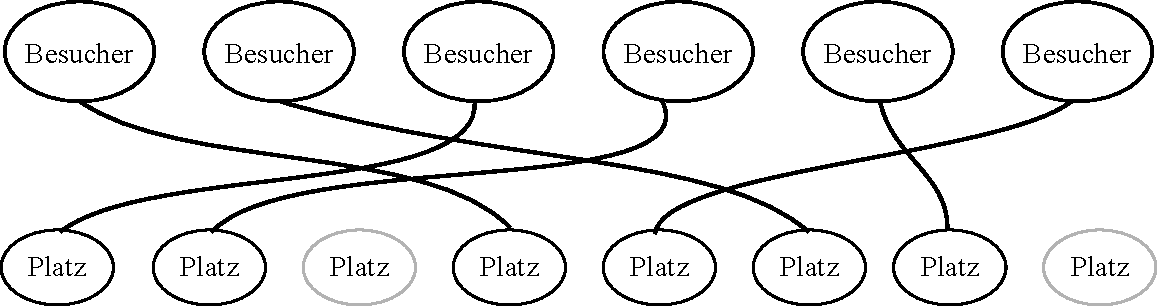
\includegraphics[scale=0.5]{Kinoabbildungen.pdf}
	\end{figure}

	\textbf{Achtung:} Das dient nur der Veranschaulichung und ist \textbf{keine} Möglichkeit, eine Abbildung formal anzugeben!
\end{frame}

%\begin{frame}
%	\frametitle{Lösung}
%	\textit{In dieser Teilaufgabe nehmen wir an, 6 Kinobesucher besuchten ein Kino mit 8 Plätzen. Wie viele injektive Abbildungen gibt es?} \\[2em] \pause
%	
%	Es gibt insgesamt $$8 \cdot 7 \cdot 6 \cdot 5 \cdot 4 \cdot 3 = 20160$$ injektive Abbildungen. \\[1em]
%	Der erste Besucher hat 8 Plätze zur Auswahl. Da aufgrund der Injektivität der nächste Besucher einen anderen Sitzplatz wählen muss, stehen ihm noch 7 Plätze zur Auswahl. Dies kann man für die restlichen Besucher fortsetzen.
%	
%\end{frame}

\subsection{Aufgabe 2}
\begin{frame}{Aufgabe 2}
	
	Was kann man über die Surjektivität, Injektivität und Bijektivität folgender Abbildungen sagen? Begründet jeweils kurz.
	\visible<+(-1)>{}
	\begin{alist}
		\item $f \from \R \functionto \R, \; x \mapsto x^2$ \\
		\visible<+-|handout:2->{
			Weder injektiv ($f(-2) = f(2) = 4$) noch surjektiv (auf $-1 \in \R$ wird nicht abgebildet) \impl auch nicht bijektiv.
		}
		\item $f \from \R_+ \functionto \R_+, \; x \mapsto x^2$ \\
		\visible<+-|handout:2->{
			Wir können zu jedem $y \in \R_+$ ein $x \in \R_+$ angeben, so dass $f(x) = y$, nämlich $ x = \sqrt{\mathstrut y}$. \\
			\impl surjektiv, und da dieses $x$ eindeutig ist auch injektiv \impl bijektiv.
		}
		
		\item $f \from \N_0 \functionto \N_0, \; x \mapsto \casesl{ 42 & \text{wenn $x = 0$} \\ x - 1 & \text{sonst} }$ \\
		\visible<+-|handout:2->{
			Nicht injektiv ($f(0) = f(43) = 42$), aber surjektiv (Für jedes $x \in \N_0$ gilt: $x + 1 \in \N_0 \text{ und } f(x+1) = x$) \\ \impl nicht bijektiv.
		} 
	\end{alist}
\end{frame}



%\begin{frame}[t]
%	\begin{block}{Wahr oder Falsch?}
%		Sei $M$ eine beliebige endliche Menge und $f$ eine Abbildung $f \from M \functionto M$. \\
%			\TrueQuestion{Wenn $f$ injektiv ist, dann ist $f$ auch surjektiv.}
%			\TrueQuestion{Wenn $f$ surjektiv ist, dann ist $f$ auch injektiv.}
%			\FalseQuestionE{Die beiden Aussagen gelten auch, wenn $M$ nicht endlich ist.}{Gegenbeispiele: \\ 
%				$f \from \N_0 \functionto \N_0, n \mapsto 2 \* n $ \\ 
%				$g \from \N_0 \functionto \N_0, n \mapsto \floor{\dfract n/2 }$}
%	\end{block}
%	
%\end{frame}